\subsection{Berechnung der Diskreten Fouriertransformation mittels FFT}\label{sec:BerechnungFFT}
Die Mathematiker Cooley und Tukey haben einen Algorithmus entwickelt und im Jahr 1965 veröffentlich, mit dem sich die \gls{dft} mit vergleichsweise wenig Multiplikationen
und somit deutlich schneller als bei der allgemeinen \gls{dft} berechnen lässt. Das Verfahren wird als \gls{fft} bezeichnet.
Grundlage ist, dass sich eine DFT
in kleinere Teil-DFTs aufspalten lässt, welche durch Ausnutzen von Symmetrieeigenschaften in der Summe weniger Koeffizienten haben. 
Üblich ist die Radix-2 FFT, Ausgangspunkt ist also eine DFT mit 2 Eingangswerten.
Da mit jeder weiteren Teil-DFT sich die Anzahl der Eingangswerte verdoppelt, eignet sich diese Methode nur für Eingangsvektoren der Größe $2^n$. Dieser
vermeindliche Nachteil lässt sich durch Auffüllen des Eingangsvektors mit Nullen (Zeropadding) eliminieren. Dies hat zur Folge, dass die Größe des Ausgangsvektors
immer eine Potenz von zwei ist. Abbildung \ref{pic:Butterfly} illustriert dies anhand eines Eingangsvektors mit acht Werten. 
Um diesen Algorithmus anwenden zu können ist es erforderlich, dass die Werte im Eingangsvektor in umgekehrte Bitreihenfolge getauscht werden (bitreversed order).
Dies geschieht nach dem Muster, dass die Indizes der Eingangswerte, wie
üblich bei 0 beginnend, binär dargestellt werden. Nun wird die Reihenfolge der Bits getauscht. Auf diese Weise tauschen bei einem 8-Bit Vektor die
Elemente 2 und 5 sowie 4 und 7 ihre Position.

Aus Gleichung (\ref{eq:Twiddlefaktorenberechnung}) ist 
bekannt, dass die Variablen der Twiddlefaktorberechnung die Indizes der Eingangs- sowie Ausgangsvektoren sind. Hieraus lässt sich bereits erkennen, dass
die gesamte Twiddlefaktormatrix N verschiedene komplexe Werte enthält. Dies wird auch aus Abbildung \ref{pic:Einheitskreis_Faktoren} aus Abschnitt 
\ref{sec:AnalyseBewertungTwiddlefaktornMatrizen} am Beispiel für N=8 ersichtlich. Darüber hinaus lässt sich erkennen, dass die komplexen Zeiger den Einheitskreis 
in N Bereiche mit einem Winkel von $\frac{2 \pi}{N}$ unterteilen. Bekannt ist ebenfalls, dass der erste Wert immer die $1$ ist.
Daraus ergibt sich bei einer DFT mit 2 Eingangswerten die Twiddlefaktoren $1$ und $-1$, sodass eine Multiplikation entfällt. 

Ähnlich verhält es sich mit der zweiten Stufe.
Hier ergeben sich die Werte $1, -j, -1, j$, was ebenfalls bedeutet, dass keine Multiplikation erfolgen muss. Der Zweite Schritt zur Reduzierung des Rechenaufwandes ergibt sich
aus der Erkenntnis, dass die Werte $exp(-i 2 \pi m n/N)$ und $exp(-i 2 \pi \frac{m n}{2}/N) = -exp(-i 2 \pi m n/N)$ lediglich ein negiertes Vorzeichen haben. Auch dies lässt sich der Abb. 
(\ref{pic:Einheitskreis_Faktoren}) entnehmen. Auf diese Weise fällt der Faktor $-j$ weg. Bedeutend wichtiger ist jedoch, dass sich so die Hälfte der Multiplikationen einsparen lässt.

Bei der dritten Stufe gibt es wegen der acht Eingangswerte theoretisch auch acht Faktoren. Aus den genannten Symmentriegründen halbiert sich die Anzahl. Wiederum die Hälfte davon 
sind komplexe Faktoren, die übrigen erfordern keine Multiplikation. Dies bedeutet, dass zwei komplexe Multiplikationen durchgeführt werden müssen, was wiederum insgesamt acht reellen 
Multiplikationen entspricht. 


Wie gezeigt wurde, werden nur zwei komplexe Multiplikationen benötigt. Eine Abschätzung der benötigten komplexen Multiplikationen erhält man mit der Gleichung (\ref{eq:FFT_komplexMult}):

\begin{equation}\label{eq:FFT_komplexMult}
 \frac{N}{2}\log_2(N) = \frac{8}{2}\cdot 3 = 12
\end{equation}

Insbesondere bei größeren FFTs ist die relative Abweichung bedeutend geringer.


\begin{figure}[htbp]
 \centering
 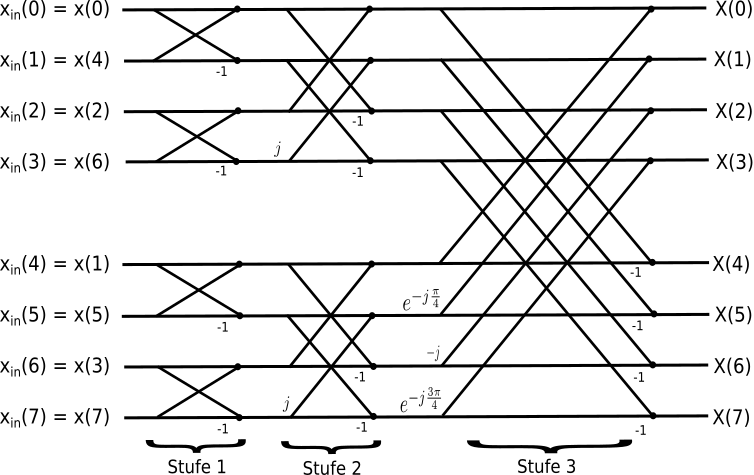
\includegraphics[width=0.7\textwidth]{img/Butterfly.png}
 \caption{Berechnungsschema der DFT mit 8 Eingangswerten nach dem Butterfly-Verfahren}
 \label{pic:Butterfly}
\end{figure}


